\section{Control de Formaciones en Sistemas No Holonómicos}
\onecolumn
\subsection{Efecto Látigo y Noción de Ancla Virtual}
Error de formación sobre errores relativos, con atracción al ancla virtual:
\begin{equation*}
    \mathbf{e}_i =
    \underbrace{-\sum_{j \in \mathcal{N}_i} a_{ij}\big[(\mathbf{x}_i-\mathbf{r}_i)-(\mathbf{x}_j-\mathbf{r}_j)\big]}_{\text{\footnotesize Consenso entre vecinos}}
    \;\;
    \underbrace{-\,\beta\, b_i^0\big[(\mathbf{x}_i-\mathbf{r}_i)-\mathbf{x}_0\big]}_{\text{\footnotesize Atracción al ancla virtual}}
\end{equation*}

Como cada seguidor persigue una posición referida al ancla virtual, un giro brusco de esta se propaga en cadena y se amplifica hacia los extremos de la formación: el efecto látigo.
\begin{figure}[H]
    \centering
    
\includegraphics[width=0.9\textwidth]{/home/calafaker/Control-Formation/documentacion/figuras/personales/formacion_v_gazebo.pdf}
    \caption{Formación en V con ancla virtual en Gazebo: trayectorias y evolución del error de formación de los seguidores en cada giro del ancla virtual}
    \label{fig:consensus_results}
\end{figure}



\section{Control de Formaciones en Sistemas No Holonómicos }
\subsection{Estructura Virtual con Generador de Trayectorias}

Como en la capa maestra de Siwek~\cite{siwek2024consensus}, un generador de trayectorias mueve la estructura virtual y cada robot rastrea su lugar dentro de ella:

\begin{figure}[H]
\centering
\ifshow
    \animategraphics[autoplay,loop,height=3.8cm]{10}{Pics/vs_frames/vs-}{0}{743}
\else
    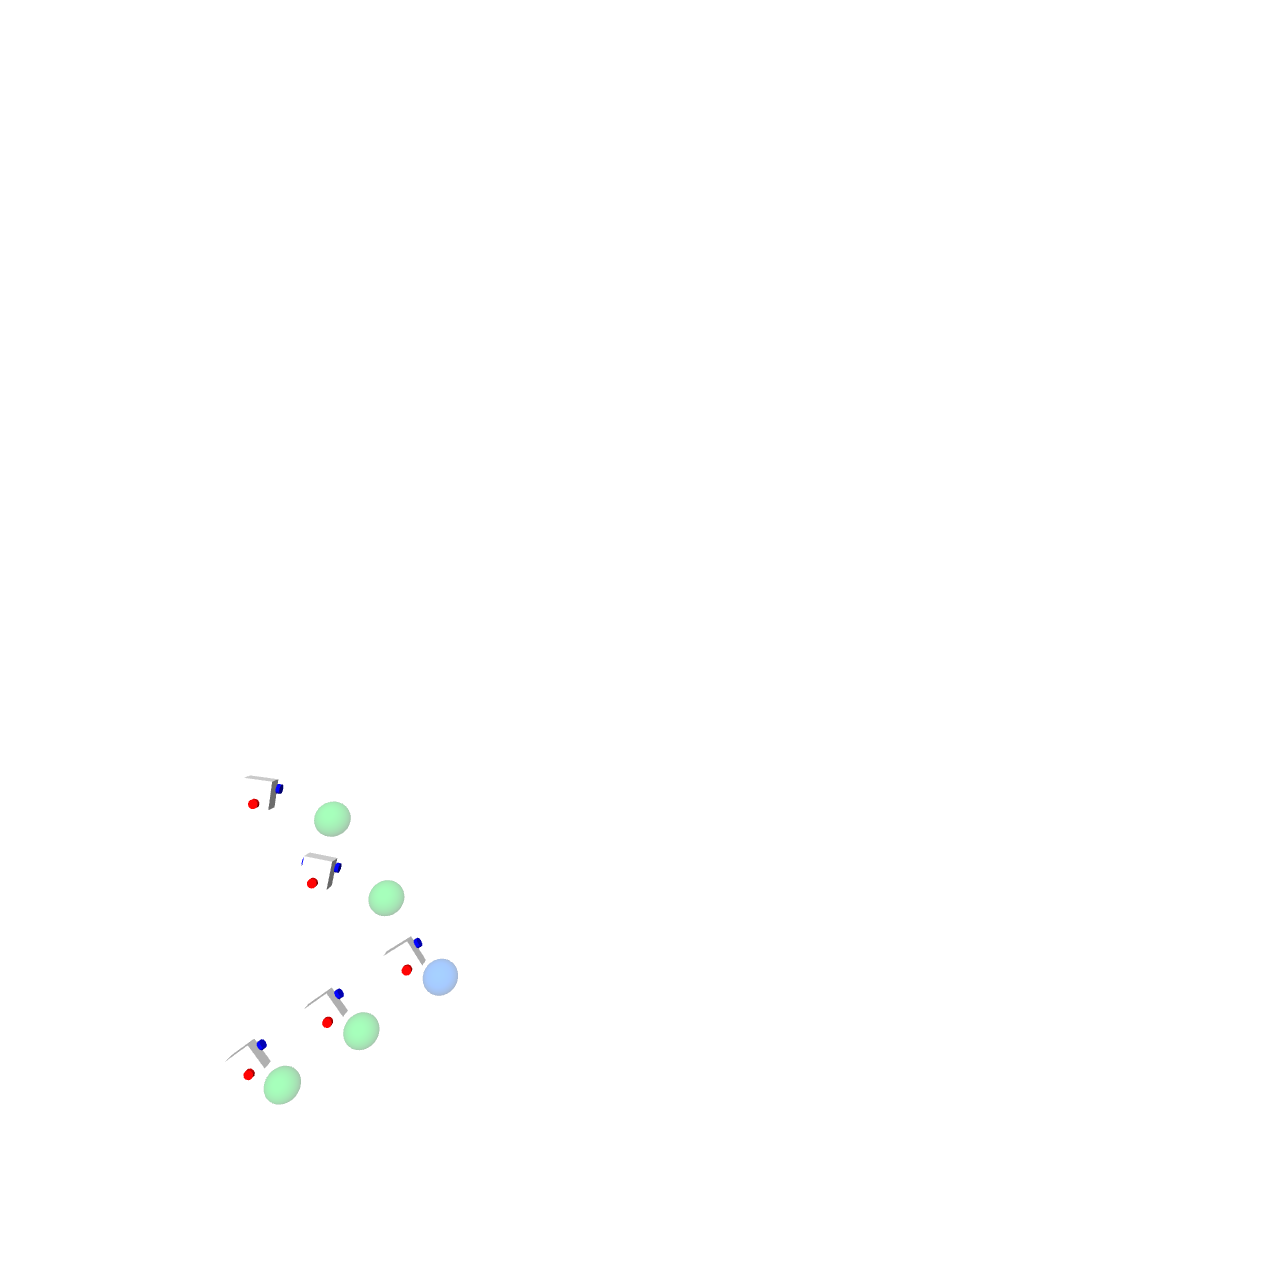
\includegraphics[height=3.8cm]{Pics/vs_frames/vs-370.png}
\fi
\caption{Simulación en Gazebo de la estructura virtual siguiendo su trayectoria}
\end{figure}
